\documentclass{article}
\usepackage{titling}
\usepackage{lipsum}
\usepackage{amsmath}
\usepackage{listings}
\usepackage{graphicx}
\usepackage{subcaption}
\usepackage{pgfplots}
\usepackage{float}
\usepackage[margin=1in]{geometry}
\usepgfplotslibrary{statistics}



\begin{document}
\noindent
\begin{minipage}[t]{0.6\textwidth}
    \begin{flushleft}
        \LARGE\textbf{Math 343 - Homework 4} \\
        \vspace{6pt} % add 6pt of vertical space
        \hrule width 10cm
        \vspace{12pt}
        \large\textbf{Preston Duffield} \\
        \large Western Washington University \\
        \today
        % April 18, 2023
        \vspace{24pt}
    \end{flushleft}
\end{minipage}

\section*{Question 1}

\subsection*{a)}
\begin{figure}[H]
    \centering
    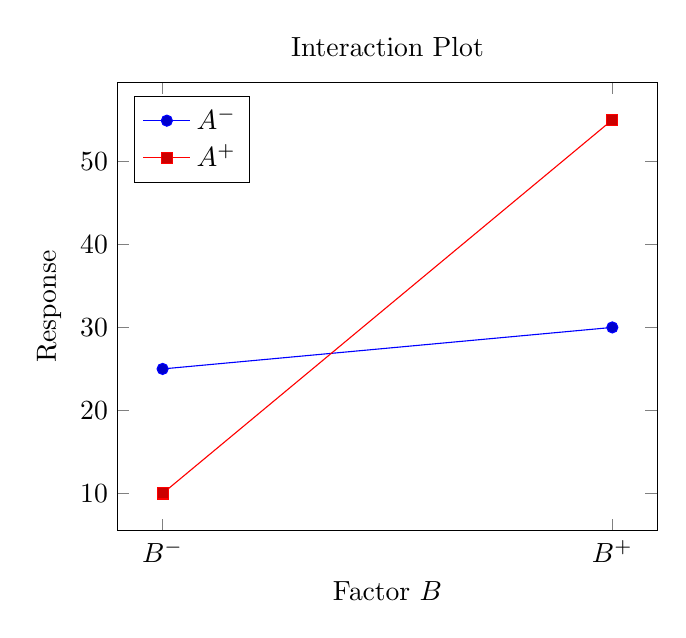
\begin{tikzpicture}
        \begin{axis}[
            title={Interaction Plot},
            xlabel={Factor $B$},
            ylabel={Response},
            symbolic x coords={$B^{-}$, $B^{+}$},
            xtick=data,
            legend pos=north west
        ]
        \addplot coordinates {($B^{-}$, 25) ($B^{+}$, 30)};
        \addplot coordinates {($B^{-}$, 10) ($B^{+}$, 55)};
        \legend{$A^{-}$,$A^{+}$}
        \end{axis}
    \end{tikzpicture}
    \caption{ An interaction plot for a $2^2$ factorial design. Since the Lines in the interaction plot are not parallel, this indicates interaction. }
\end{figure}


\subsection*{b)}
\begin{flushleft}
The Main Effect of $A$ is:
\end{flushleft}
\begin{align*}
    A & = \bar{y}_{A^{+}} - \bar{y}_{A^{-}} \\
      & = \frac{\mu_{22} + \mu_{21}}{2} - \frac{\mu_{12} + \mu_{11}}{2} \\
      & = \frac{55 + 10}{2} - \frac{30 + 25}{2} \\
      & = 5
\end{align*}
\begin{flushleft}
The Main Effect of $B$ is:
\end{flushleft}
\begin{align*}
    B & = \bar{y}_{B^{+}} - \bar{y}_{B^{-}} \\
      & = \frac{\mu_{12} + \mu_{22}}{2} - \frac{\mu_{11} + \mu_{21}}{2} \\
      & = \frac{30 + 55}{2} - \frac{25 + 10}{2} \\
      & = 25
\end{align*}
\clearpage
\begin{flushleft}
The Interaction Effect of $A$ and $B$ is:
\end{flushleft}
\begin{align*}
    AB & = \frac{\mu_{22} + \mu_{11}}{2} - \frac{\mu_{21} + \mu_{12}}{2} \\
       & = \frac{55 + 25}{2} - \frac{10 + 30}{2} \\
       & = 20
\end{align*}

\section*{Question 2}

\subsection*{a)}



\begin{figure}[H]
    \title{test}
    \centering
    \textbf{Two-way ANOVA: y versus, A, B} \\
    \begin{equation*}
        \begin{array}{c|c|c|c|c|c}
            \text{Source} &\text{DF}& \text{SS} & \text{MS} & \text{F} &\text{P}  \\
            \hline
            \text{A}            & \text{1}   & \text{0.322}   & \textbf{0.322}      & \textbf{0.0366}  &\textbf{0.098}  \\
            \text{B}            & \textbf{2} & \text{80.554}  & \text{40.2771}  & \text{4.59} &\textbf{0.171}  \\
            \text{Interaction}  & \textbf{2} & \textbf{45.348}     & \textbf{22.674}      & \textbf{2.5832}  &\textbf{0.031}  \\
            \text{Error}        & \text{12}  & \text{105.327} & \text{8.7773}   &   &  \\
            \text{Total}        & \text{17}  & \text{231.551} &  &  &  \\
        
        \end{array}
        \end{equation*}\\
    \caption{ Two-way ANOVA: y versus, A, B. Note that calculated values are bold. }
\end{figure}

\subsection*{b)}
3 levels where used for Factor B.
\subsection*{c)}
18 total observations of the experiment were performed.
\subsection*{d)}
\begin{flushleft}
    \textbf{Interaction:} \\
    $H_0$: $(\tau \beta)_{11} = (\tau \beta)_{12} = (\tau \beta)_{22} = (\tau \beta)_{21} = (\tau \beta)_{13} = (\tau \beta)_{23} = 0$ \\
    $H_a$: At least one $(\tau \beta)_{ij}$ is different.\\
\end{flushleft}

Since the p-value for the interaction of the two factors is $0.031 < \alpha = 0.05$, we can conclude the following.
There is enough evidence to support the hypotheis that at least one $(\tau \beta)_{ij}$ is different,
ie, there exists interaction between the two factors.


\begin{flushleft}
    \textbf{Factor A:}\\
    $H_0$: $\tau_1 = \tau_2 = 0$ \\
    $H_a$: At least one $\tau_i$ is different.\\
\end{flushleft}

Since the p-value is $0.098 > \alpha = 0.05$, we can conclude the following. \\
There is not enough statistic evidence to support at least one $\tau_i$ being different.


\begin{flushleft}
    \textbf{Factor B:} \\
    $H_0$: $\beta_1 = \beta_2 = \beta_3 = 0$ \\
    $H_a$: At least one $\beta_i$ is different.\\
\end{flushleft}

Since the p-value is $0.171 > \alpha = 0.05$, we can conclude the following. \\
There is not enough statistic evidence to support at least one $\beta_i$ being different.

\clearpage
\section*{Question 3}

\subsection*{b)}

% \begin{figure}[h]
%     \centering
%     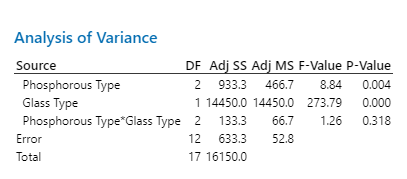
\includegraphics[width=0.5\textwidth]{./images/3_b.png}
%     \caption{Anova table from Minitab.}
%     \label{fig:3_B}
% \end{figure}
% \begin{figure}[h]
%     \centering
%     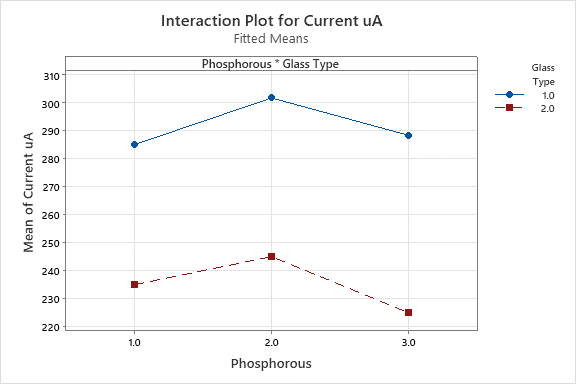
\includegraphics[width=0.5\textwidth]{./images/3_b_2.png}
%     \caption{Anova table from Minitab.}
%     \label{fig:3_b_2}
% \end{figure}

\begin{figure}[h]
    \centering
    \begin{subfigure}[b]{0.4\textwidth}
        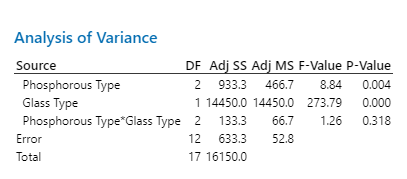
\includegraphics[width=1\textwidth]{./images/3_b.png}
        \caption{Anova table from Minitab.}
      \label{fig:img1}
    \end{subfigure}
    \hfill
    \begin{subfigure}[b]{0.5\textwidth}
        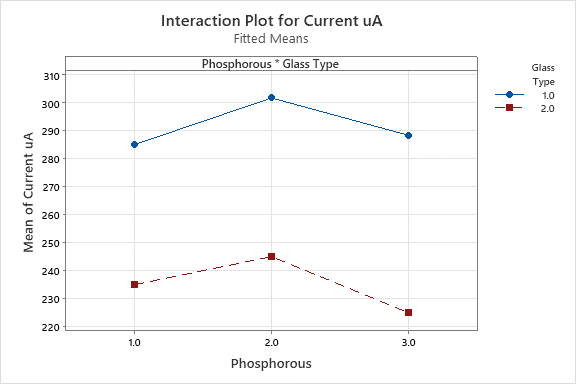
\includegraphics[width=1\textwidth]{./images/3_b_2.png}
        \caption{Interaction plot from Minitab.}
      \label{fig:img2}
    \end{subfigure}
    \label{fig:both}
\end{figure}

\begin{flushleft}
    $H_0$: $(\tau \beta)_{11} = (\tau \beta)_{12} = (\tau \beta)_{22} = (\tau \beta)_{21} = (\tau \beta)_{32} = (\tau \beta)_{31} = 0$ \\
    $H_a$: At least one $(\tau \beta)_{ij}$ is different.\\
\end{flushleft}

Since the p-value for the interaction of the two factors is $0.318 > \alpha = 0.05$, we can conclude the following.
There is not enough evidence to support the hypotheis that at least one $(\tau \beta)_{ij}$ is different,
ie, there does not exist interaction between the two factors. 


\subsection*{c)}
\begin{figure}[h]
    \centering
    \begin{subfigure}[b]{0.45\textwidth}
        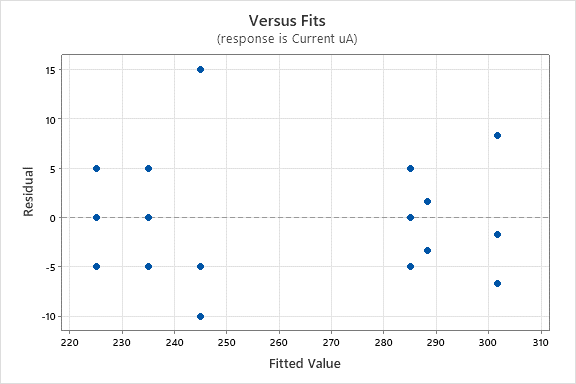
\includegraphics[width=1\textwidth]{./images/3_c_1.png}
        \caption{Residuals versus fits plot from Minitab.}
      \label{fig:img11}
    \end{subfigure}
    \hfill
    \begin{subfigure}[b]{0.45\textwidth}
        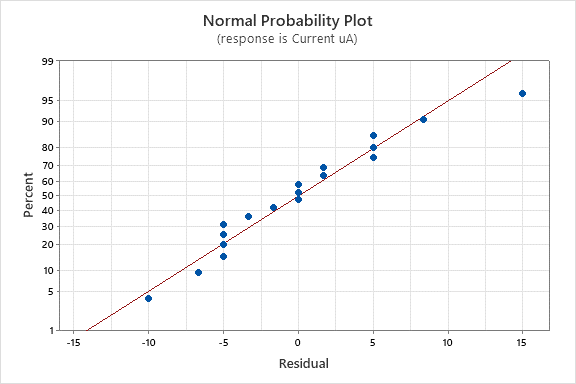
\includegraphics[width=1\textwidth]{./images/3_c_2.png}
        \caption{Normal probability plot from Minitab.}
      \label{fig:img22}
    \end{subfigure}
    \label{fig:both}
\end{figure}
The residual plot does not seem to indicate heteroskedasticity. The normal probability plot appears to follow a stright line, indicating normality.
These two plots indicate that the model assumptions are satified.
\subsection*{d)}
\begin{flushleft}
    $H_0$: $\tau_1 = \tau_2 = \tau_3 = 0$ \\
    $H_a$: At least one $\tau_i$ is different.\\
\end{flushleft}
Since the p-value is $0.004 < \alpha = 0.05$, we can conclude the following. \\
There is enough statistic evidence to support at least one $\tau_i$ being different.
% This is significant so do a tukeys pairwise.
\\
\textbf{Tukey's test for pairwise comparison} \\
First we calulate the means of the Phosphorous Types: \\
\begin{equation*}
    \begin{array}{c|c}
        \text{Phosphorous Type} & \text{Mean} \\
        \hline
        1 &  \frac{285+235}{2} = 260\\
        2 &  \frac{301.67+245}{2} = 273.335\\
        3 &  \frac{288.33+225}{2} = 256.665\\
    
    \end{array}
    \end{equation*}\\
\begin{flushleft}
Then we calculate $\alpha$ from the $FWE = 0.05$: \\
\end{flushleft}
$\alpha = 1 - (1- 0.05)^{\frac{1}{6}} = 0.0085$

\begin{flushleft}
    Then note that: \\
    \end{flushleft}
\begin{align*}
    q_{\alpha , a , df_{error}}\sqrt{\frac{MSE}{b \cdot n}} & = q_{0.0085 , 3 , 12}\sqrt{\frac{52.8}{2 \cdot 6}} \\
    & = 5.17 \cdot 2.0976 \\
    & = 10.85
\end{align*}


\begin{flushleft}
    The difference in means are:
\end{flushleft}
\begin{equation*}
    \begin{array}{c|c|c}
        \text{Difference of Types} &\text{Difference}&95\% \text{Simultaneous C.I.}\\
        \hline
        2 - 1 & 273.335 - 260 = 13.335 & (2.48, 24.16)\\
        3 - 1 & 256.665 - 260 = -3.335 & (-14.18, 7.51)\\
        3 - 2 & 256.665 - 273.335 = -16.67 & (-33.34, -5.81)\\
    
    \end{array}
    \end{equation*}\\
\begin{flushleft}
    Since the C.I. for the difference in means 3 and 1 contains 0, we can say that the means are not significantly different. The line graph representing the data is as follows:
\end{flushleft}

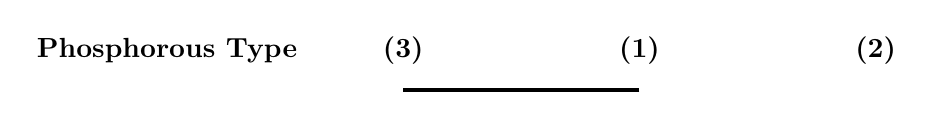
\begin{tikzpicture}[yscale=-1]
    % Define the positions of the labels
    \coordinate (labelPos) at (0, 0);
    \coordinate (3Pos) at (3, 0);
    \coordinate (1Pos) at (6, 0);
    \coordinate (2Pos) at (9, 0);

    % Draw the labels
    \node at (labelPos) {\textbf{Phosphorous Type}}; % Treatment label
    \node at (3Pos) {\textbf{(3)}};
    \node at (1Pos) {\textbf{(1)}};
    \node at (2Pos) {\textbf{(2)}};

    % Draw the line
    \draw[ultra thick] ([yshift=0.5cm]1Pos) -- ([yshift=0.5cm]3Pos);
    % \draw[thick] ([yshift=1cm]1Pos) -- ([yshift=1cm]2Pos); % another theoretical line.
\end{tikzpicture}

\subsection*{e)}
For a Fisher's LSD 95\% confidence
interval for difference in mean between Phosphor Type 1 and Phosphorous Type 2.
First we note the difference in means $\beta_j - \beta_{j`} = 260 - 273.33 = -13.33$.
% We can say the 2 treatment means are significantly different if:
% \begin{align*}
%     \left| \bar{y}_{i} - \bar{y}_{j} \right| &> t_{\alpha/2, N-a} \sqrt{MSE \cdot \left( \frac{1}{n_i} + \frac{1}{n_j} \right)} \\
%     \left| 260 - 273.33 \right|  &> t_{0.025, 18-3} \sqrt{5.28 \cdot \left( \frac{2}{6} \right)} \\
%     13.33 &> 2.131 \cdot 1.326 \\
%     13.33 &> 2.825
% \end{align*}
% Therefore, via Fisher's LSD method, The means for Phosphorous Types 1 and 2 are significantly different.
\begin{align*}
    -13.33 &\pm t_{\alpha/2, df_{error}} \sqrt{\frac{2 \cdot MSE}{a \cdot n}} \\
           &\pm t_{0.025, 12} \sqrt{\frac{2 \cdot 52.8}{3 \cdot 18}} \\
           &\pm 2.179 (1.3984) \\
           &\pm 3.047
\end{align*}
We are 95\% confident that the true difference in means for Phosphorous Types 1 and 2 is between -16.377 and -10.283.

\clearpage
\section*{Question 4}
\subsection*{a)}
\begin{figure}[h]
    \centering
    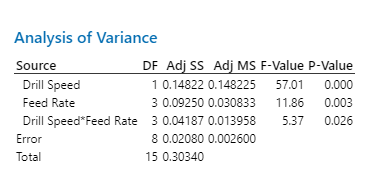
\includegraphics[width=0.5\textwidth]{./images/4_a.png}
    \caption{Anova table from Minitab.}
    \label{fig:3_b_2}
\end{figure}

\subsection*{b)}

\begin{figure}[h]
    \centering
    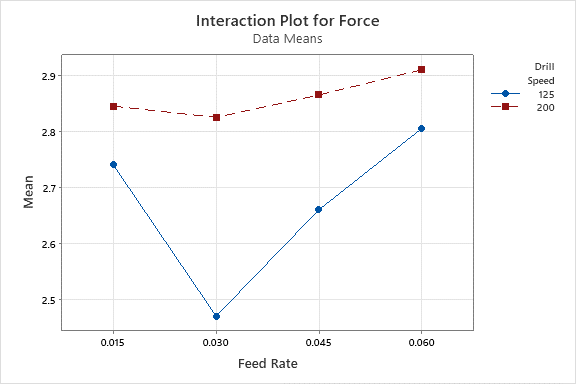
\includegraphics[width=0.5\textwidth]{./images/4_b.png}
    \caption{Interaction plot from Minitab.}
    \label{fig:3_b_2}
\end{figure}

Based on the interaction plot, since the lines are not parallel, there does appear to be interaction between the 2 factors.

\subsection*{c)}
\begin{flushleft}
    $H_0$: There does not exist interaction between the two factors. \\
    $H_a$: There does exist interaction between the two factors.\\
\end{flushleft}

Since the p-value for the interaction of the two factors is $0.026 < \alpha = 0.05$, we can conclude the following.
There is enough evidence to support the hypotheis that there does exist interaction between the two factors. 
\subsection*{d)}

\textbf{Tukey's test for pairwise comparison at FWE = 0.05} \\
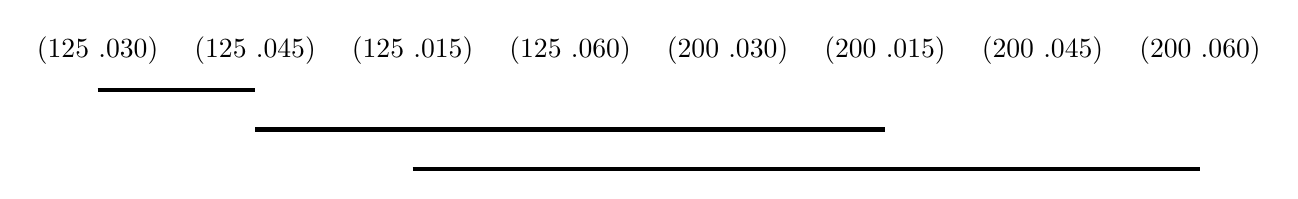
\begin{tikzpicture}[yscale=-1]
    % Define the positions of the labels
    \coordinate (labelPos) at (0, 0);

    \coordinate (1Pos) at (2, 0);
    \coordinate (2Pos) at (4, 0);
    \coordinate (3Pos) at (6, 0);
    \coordinate (4Pos) at (8, 0);
    \coordinate (5Pos) at (10, 0);
    \coordinate (6Pos) at (12, 0);
    \coordinate (7Pos) at (14, 0);
    \coordinate (8Pos) at (16, 0);

    % Draw the labels
    % \node at (labelPos) {\textbf{Drill Speed $\times$ Feed Rate }}; % Treatment label
    
    \node at (1Pos) {\text{(125 .030)}};
    \node at (2Pos) {\text{(125 .045)}};
    \node at (3Pos) {\text{(125 .015)}};
    \node at (4Pos) {\text{(125 .060)}};
    \node at (5Pos) {\text{(200 .030)}};
    \node at (6Pos) {\text{(200 .015)}};
    \node at (7Pos) {\text{(200 .045)}};
    \node at (8Pos) {\text{(200 .060)}};


    % Draw the line
    \draw[ultra thick] ([yshift=0.5cm]1Pos) -- ([yshift=0.5cm]2Pos);
    \draw[ultra thick] ([yshift=1cm]2Pos) -- ([yshift=1cm]6Pos);
    \draw[ultra thick] ([yshift=1.5cm]3Pos) -- ([yshift=1.5cm]8Pos);
    
    
\end{tikzpicture}
\subsection*{e)}
\textbf{Fisher's LSD 95\% C.I for the difference in treatment means} \\
The mean for Drill Speed = 125, Feed Rate = 0.015, $\bar{y}_{125, 0.015} = 2.740$. \\
The mean for Drill Speed = 200, Feed Rate = 0.045, $\bar{y}_{200, 0.045} = 2.865$. \\
The value of their difference is $2.740 - 2.865 = -0.125$.
% \begin{flushleft}
% The two treatment means are significantly different if:
% \end{flushleft}
% \begin{align*}
%     0.125 &> t_{\alpha/2, df_{error}}\sqrt{\frac{2 MSE}{n}} \\
%           &> t_{0.025, 8}\sqrt{\frac{2 \cdot 0.0026}{2}} \\
%           &> 2.306 \cdot 0.0509 \\
%           &> 0.1173
% \end{align*}
% \begin{flushleft}
% Therfore, the two treatment means $\bar{y}_{125, 0.015}$ and $\bar{y}_{200, 0.045}$ are significantly different at $\alpha = 0.05$
% \end{flushleft}
\begin{align*}
    -0.125 &\pm t_{\alpha/2, df_{error}} \sqrt{\frac{2 \cdot MSE}{n}} \\
           &\pm t_{0.025, 8} \sqrt{\frac{2 \cdot 0.0026}{16}} \\
           &\pm 2.306 (0.018) \\
           &\pm 0.041
\end{align*}
We are 95\% confident that the true difference in means for Drill Speed = 125, Feed Rate = 0.015 and Drill Speed = 200, Feed Rate = 0.045
is between -1.166 and -1.084.


\section*{Question 5}
\subsection*{d)}
For the model: $y = \beta_0 + \beta_1 x_1 + \beta_2 x_2 + \beta_{22} x^{2}_2 + \beta_{12} x_1 x_2 + \epsilon$

The coefficients are:
\begin{equation*}
    \begin{array}{c|c|c|c}
        \text{Coefficient} &\text{Value} &\text{P-value} &\text{Significant at } \alpha = 0.05\text{?}\\
        \hline
        \beta_0  & -977.5     & 0.000 & Yes\\
        \beta_1  & -10.64     & 0.013 & Yes\\
        \beta_2  & 2.028      & 0.000 & Yes\\
        \beta_22 & -0.001040  & 0.000 & Yes\\
        \beta_12 & 0.01060    & 0.016 & Yes
    
    \end{array}
    \end{equation*}\\

Since each coefficient is significant at $\alpha = 0.05$.
The model $y = \beta_0 + \beta_1 x_1 + \beta_2 x_2 + \beta_{22} x^{2}_2 + \beta_{12} x_1 x_2 + \epsilon$ is supported by the experiment.

\begin{figure}[h]
    \centering
    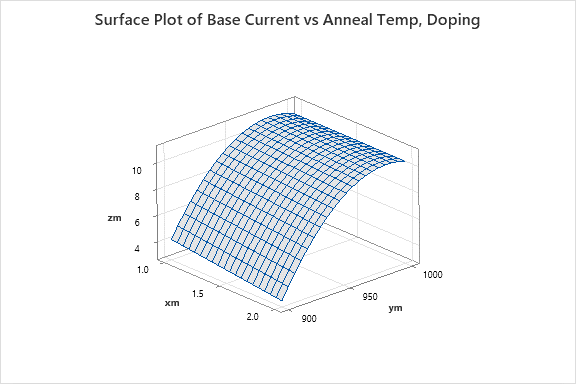
\includegraphics[width=0.6\textwidth]{./images/5_d.png}
    \caption{Surface plot from Minitab.}
    \label{fig:3_b_2}
\end{figure}

\section*{Question 6}

\subsection*{a)}
\begin{figure}[h]
    \centering
    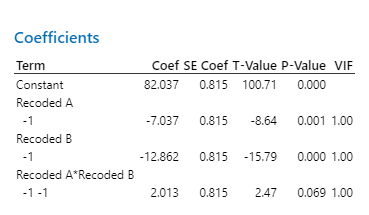
\includegraphics[width=0.5\textwidth]{./images/6_a_1.png}
    \caption{Coefficients from Minitab.}
    \label{fig:3_b_2}
\end{figure}

\begin{figure}[h]
    \centering
    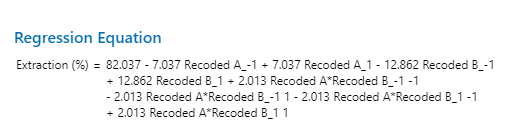
\includegraphics[width=0.7\textwidth]{./images/6_a_2.png}
    \caption{Regression equation from Minitab.}
    \label{fig:3_b_2}
\end{figure}

% Thus the regression model is:
% $y = 64.15 + 10.05 x_1 + 21.70 x_2 + 8.05 x_1 x_2$
\subsection*{b)}
\begin{flushleft}
The estimated main effect of A is:
\end{flushleft}
\begin{align*}
    A &= 2 \hat{\beta}_1\\
      &= 2(10.05)\\
      &= 20.10
\end{align*}
\begin{flushleft}
The estimated main effect of B is:
\end{flushleft}
\begin{align*}
    B &= 2 \hat{\beta}_2\\
      &= 2(21.70)\\
      &= 43.40
\end{align*}
\begin{flushleft}
The estimated interaction effect of A and B is:
\end{flushleft}
\begin{align*}
    AB &= 2 \hat{\beta}_3\\
       &= 2(8.05)\\
       &= 16.10
\end{align*}


\clearpage
\subsection*{c)}

\begin{figure}[h]
    \centering
    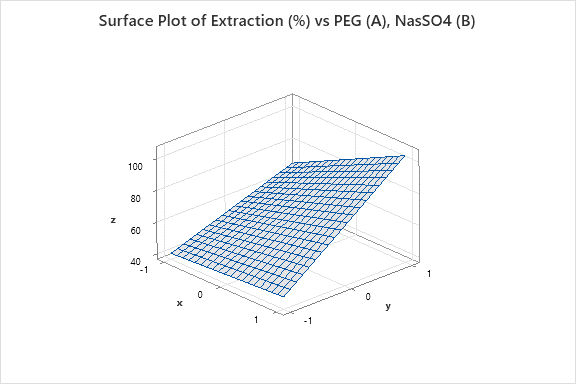
\includegraphics[width=0.7\textwidth]{./images/6_c.png}
    \caption{Regression equation from Minitab.}
    \label{fig:3_b_2}
\end{figure}

Since there is very little curvature, interaction is likely very small. However, there is curvature, so the interaction may be significant.

\section*{Question 7}
\begin{flushleft}
In terms of these means, $\mu_{(1)}, \mu_a, \mu_b$, and $\mu_{ab}$ are the overall mean,
the effect of factor A, the effect of factor B, and the interaction effect respectively:\\
\end{flushleft}
\begin{align*}
    \mu_{(1)} &= \frac{(\mu_{11} + \mu_{21} + \mu_{12} + \mu_{22})}{4}\\
    \mu_a &= \frac{(\mu_{21} + \mu_{22})}{2} - \frac{(\mu_{11} + \mu_{12})}{2}\\
    \mu_b &= \frac{(\mu_{12} + \mu_{22})}{2}- \frac{(\mu_{11} + \mu_{21})}{2}\\
    \mu_{ab} &= \frac{(mu_{11} + mu_{22})}{2} - \frac{(mu_{21} + mu_{12})}{2}
\end{align*}
\begin{flushleft}
The intercept $\beta_0$ is the expected value of y when all factors are at their low level
(i.e., $x_1 = x_2 = -1$), which corresponds to $\mu_{11}$.
However, we must also account for the changes in y due to the other terms
in the regression model, which are non-zero when the factors are at their low level.
In other words, $\beta_0 = \mu_{11} + \beta_1 + \beta_2 + \beta_3$. \\
\end{flushleft}
\begin{flushleft}
Expressing $\beta_1, \beta_2,$ and $\beta_3$ in terms of the factor-level means, we can substitute these expressions into the equation for $\beta_0$:
$\beta_1 = \frac{\mu_a}{2}$, 
$\beta_2 = \frac{\mu_b}{2}$, and 
$\beta_3 = \frac{\mu_{ab}}{2}$.
\end{flushleft}
\begin{align*}
    \beta_0 &= \mu_{11} + \frac{\mu_a}{2} + \frac{\mu_b}{2} + \frac{\mu_{ab}}{2}\\
            &= \mu_{(1)} - \frac{\mu_{ab}}{2}
\end{align*}


\end{document}
